\documentclass[12pt]{article}
\usepackage{amsmath,amssymb,amsthm}
\usepackage[pdftex]{graphicx}
\usepackage[inline]{asymptote}
\usepackage{fancyhdr}
\usepackage[english]{babel}
\pagestyle{fancy}
\usepackage[nottoc]{tocbibind}
\usepackage{hyperref}
\usepackage{setspace}
\usepackage{csquotes}
\usepackage{multirow}
\usepackage{listings}
\usepackage{xcolor}
\usepackage{indentfirst}
\usepackage{float}
%%%%%%%%%%%%%%%%%%%%%%%%%%%%%%%%%%%%%%%%%%%
%%                                       %%
%% Students: DO NOT MODIFY THIS FILE!!!  %%
%%                                       %%
%%%%%%%%%%%%%%%%%%%%%%%%%%%%%%%%%%%%%%%%%%%

%% USAMTS style sheet
%% last modified: 23-Jul-2004

\newcounter{qnumber}

%% Student and Year/Round data
\newcommand{\realname}[1]{\newcommand{\printrealname}{#1}}
\newcommand{\username}[1]{\newcommand{\printusername}{#1}}
\newcommand{\usamtsid}[1]{\newcommand{\printusamtsid}{#1}}
\newcommand{\usamtsyear}[1]{\newcommand{\printyear}{#1}}
\newcommand{\usamtsround}[1]{\newcommand{\printround}{#1}}

%% Pagestyle setup
\setlength{\headheight}{0.75in}
\setlength{\oddsidemargin}{0in}
\setlength{\evensidemargin}{0in}
\setlength{\voffset}{-.5in}
\setlength{\headsep}{10pt}
\setlength{\textwidth}{6.5in}
\setlength{\headwidth}{6.5in}
\setlength{\textheight}{8in}
\lhead{Student: \printrealname\ \\Username: \printusername\ \\ID\#: \printusamtsid}
\chead{\Large USA Mathematical Talent Search \qquad \quad}
\rhead{\begin{tabular}[b]{|c|c|c|}\hline Year&Round&Problem\\\hline\printyear & \printround    
   &\theqnumber\\\hline\end{tabular}}
\lfoot{}
\cfoot{}
\rfoot{Page \thepage\ of Problem \theqnumber}
\renewcommand{\headrulewidth}{0.5pt}
\renewcommand{\footrulewidth}{0.3pt}
\setlength{\textwidth}{6.5in}

%% Print solutions
\newenvironment{solution}[1]{\section*{Problem #1}\setcounter{qnumber}{#1}\setcounter{page}{1}}{\eject}

\renewcommand{\baselinestretch}{1.44}



\realname{Arjun Vikram}
\username{arjvik}
\usamtsid{36783}
\usamtsyear{31}
\usamtsround{2}

\begin{document}

\begin{solution}{1} 

     \begin{asy}
        unitsize(3cm);
        
        draw((0,0)--(3,0)--(3,3)--(0,3)--(0,0));
        draw((0,1)--(3,1));
        draw((0,2)--(3,2));
        draw((1,0)--(1,3));
        draw((2,0)--(2,3));
        
        string[][] givens = {{"357","638","650"},{"50","153","338"},{"77","130","154"}};
        
        string[][] numbers = {{"14","13","15","9"},{"4","7","16","11"},{"3","1","2","10"},{"6","8","12","5"}};
        
        for(int i=0; i < 4; ++i) {
            for(int j=0; j < 4; ++j) {
                filldraw(circle((i,j),0.3), white);
                label(numbers[3-j][i], (i,j));
            }
        }

        for(int i=0; i < 3; ++i){
            for(int j=0; j < 3; ++j){
                label(givens[2-j][i], (i + 0.5, j + 0.5));
            }
        }
    \end{asy}

\end{solution}

\begin{solution}{2}
    We begin by looking at how the allowed moves change the board. Let us call
    moving the top row of blocks to the bottom \textbf{Move X} and moving the
    left column of blocks to the right \textbf{Move Y}.
    
    We notice that the order in which we perform the moves does not affect the
    ending state of the board:
    
    $$
    \begin{bmatrix}
    1 & 2 & 3 \\
    4 & 5 & 6 \\
    7 & 8 & 9 \\
    \end{bmatrix}
    \overset{{\text{Move Y}}}{\to}
    \begin{bmatrix}
    2 & 3 & 1 \\
    5 & 6 & 4 \\
    8 & 9 & 7 \\
    \end{bmatrix}
    $$
    $$
    {\small{\text{Move X}}} \downarrow
    \phantom{
    \begin{bmatrix}
    1 & 2 & 3 & 4
    \end{bmatrix}
    }
    \downarrow {\small{\text{Move X}}}
    $$
    $$
    \begin{bmatrix}
    4 & 5 & 6 \\
    7 & 8 & 9 \\
    1 & 2 & 3 \\
    \end{bmatrix}
    \overset{{\text{Move Y}}}{\to}
    \begin{bmatrix}
    5 & 6 & 4\\
    8 & 9 & 7 \\
    2 & 3 & 1\\
    \end{bmatrix}
    $$
    
    Based on this observation, we can simplify the process of performing moves
    to always perform all Move X's before Move Y's. In addition, we notice that
    performing 3 Move X's or Move Y's takes us back to where we started, so the
    only valid number of Move X's and Move Y's we need to consider are 0, 1, and 2.
    Therefore, there are only a total of 9 different states of the board after
    performing some sequence of Move X and Move Y.
    
    We also note that it is easy to make a one-is-to-one correspondence from the
    set of all colorings to a 9-bit binary number. The color of each square can
    be represented in one of the bits of the number, with 1 being lime and 0 being
    orange (or vice versa, this choice does not matter). Therefore, there are only
    $2^9=512$ possible combinations.
    
    Since there are only $9 \cdot 2^9 = 4608$ combinations of board state and colorings
    to consider, it is easy to write a Python program to determine the number of
    citrus colorings. The source code is well commented and included below.
    
    \definecolor{comment}{rgb}{0,0.4,0}
    \definecolor{string}{rgb}{0.58,0,0.82}
    \definecolor{back}{rgb}{0.95,0.95,0.95}
     
    \lstdefinestyle{prob2}{
        language=Python,
        backgroundcolor=\color{back},
        commentstyle=\color{comment},
        keywordstyle=\color{blue},
        stringstyle=\color{string},
        basicstyle=\ttfamily\footnotesize,
        breakatwhitespace=false,
        breaklines=true,
        captionpos=b,
        keepspaces=true,
        numbers=left,
        numbersep=-10pt,
        numberstyle=\color{darkgray},
        showspaces=false,
        showstringspaces=false,
        showtabs=false,
        tabsize=1,
    }
     
\lstset{style=prob2}
\begin{lstlisting}
    #!/usr/bin/env python3
    
    side_len = 3 # as given in problem statement, the grid is 3 x 3
    num_cells = side_len ** 2 # number of squares is side_len ^ 2
    
    # Define a utility function
    def unmask(num):
        """
        Takes a bitmask num, converts it into a boolean array,
        then reshapes it into a square.
        i.e. unmask(341):
         341 base 10 = 101010101 base 2
         101010101 -->  [True, False, True, False,
                               True, False, True, False, True]
                   --> [[True, False, True],
                        [False, True, False],
                        [True, False, True]]
        """
        
        # List comprehension to convert from binary number
        # to 1-dimensional boolean array
        l = [bool(num & (1<<n)) for n in range(num_cells)]
      
        # List comprehension to reshape a 1-d boolean array
        # into a 2-d square array using slices
        return [l[i:i+side_len] for i in range(0, num_cells, side_len)]
    
    # Now we are going to compute the actual answer
      
    # Counter to store the number of citrus colorings we have encountered
    citrus_count = 0
    
    # Loop over all 9-bit bitmasks to iterate over all possible colorings
    for bitmask in range(2**(num_cells)):
        # Unmask the bitmask into a square boolean array
        # True is lime, False is orange (arbitrary choice)
        coloring = unmask(bitmask)
      
        # Boolean to store whether or not our current coloring is citrus
        # Initialized to True at first, we only change it to false when
        # we prove it is not citrus
        is_citrus = True;
        
        # Begin looping through all possible states of the board
        for x_rot in range(side_len):
            # x_rot represents the number of move X we perform
        
            # x_rotated is the coloring after performing x_rot
            # of rotation X, computed via list slices
            x_rotated = coloring[x_rot:] + coloring[:x_rot]
        
            for y_rot in range(side_len):
                # y_rot represents the number of move Y we perform
        
                # y_rotated is the coloring after performing y_rot
                # of rotation Y on x_rotated, computed using
                # list slices on each sublist in a list comprehension
                y_rotated = [x_rotated[i][y_rot:] + x_rotated[i][:y_rot]
                                          for i in range(len(x_rotated))]
                # If we have performed at least one rotation, and reached
                # a coloring which is identical to the original coloring,
                # this coloring is not citrus
                if (not (x_rot == 0 and y_rot == 0)
                        and coloring == y_rotated):
                    is_citrus = False
        # If is_citrus is still true after the loop, the coloring
        # must be citrus, and we increase our counter
        if is_citrus:
            citrus_count += 1

    # We have now looped over all possible colorings, and
    # citrus_count contains the number of citrus colorings found
    print(f"Total number of citrus colorings: {citrus_count}")
\end{lstlisting}

    When this program is run, the output is
    \begin{verbatim}
        Total number of citrus colorings: 486
    \end{verbatim}
    
    There are clearly $2^9=512$ total possible colorings.
    
    Therefore, our answer is $\dfrac{486}{512} = \boxed{\dfrac{243}{256}}$.
 
    
\end{solution}

% \begin{solution}{3}
% % Solution to Problem 3 goes here
% \end{solution}

\begin{solution}{4}

    \newcommand{\jesterold}[6]{
        \underline{\text{ $#1$ }}\ 
        \underline{\text{ $#2$ }}\ 
        \underline{\text{ $#3$ }}\ 
        \underline{\text{ $#4$ }}\ 
        \underline{\text{ $#5$ }}\ 
        \underline{\text{ $#6$ }}
    }
    \newcommand{\jester}[6]{
        \underbrace{\underline{\text{ $A$ }}\ 
                    \underline{\text{ $B$ }}}_{[#3,\ #4]}\ 
        \underline{\text{ #1 }}\ \underline{\text{ #2 }}\ 
        \underbrace{\underline{\text{ $E$ }}\ 
                    \underline{\text{ $F$ }}}_{[#5,\ #6]}
    } 

    Before beginning, let us label the jesters in each group to make the solution simpler.
    When looking at a group of 6 jesters, let $A$ be the height of the shortest jester in inches,
    $B$ be the height of the second shortest jester in inches, etc, until $F$ is the height of the
    tallest of the 6 jesters in inches (i.e. when arranged in increasing order of height, they are labeled as follows):
    \begin{equation*}
        \jesterold ABCDEF
    \end{equation*}
    
    To begin, we will look at the number of candied cherries that Princess Peach will receive
    over the first 100 days. We can see that the minimum median height of any group of 6 jesters is
    $3.5\text{ in}$ (in order to minimize the median height, we want the $C$ and $D$ to be as small as possible,
    so and the smallest values are $C=3$ and $D=4$). Thus, the first day that Princess Peach will receive any candied
    cherries is on day $n=54$, where the median height is $4\text{ in}$. Now, let's focus on day $54$ for a moment.

    \subsubsection*{Day 54}
    On day $54$, the median height is $4$. In order for the median height of a group of $6$ jesters to be $4$ inches,
    $C=3$ and $D=5$ (if $C$ is reduced, $A$ and $B$ will not be positive integers, and if $C$ is increased, $D$ will
    not be distinct from $C$). Therefore, we must have the following jesters fixed in the group:
    \begin{equation*}
        \jesterold AB35EF
    \end{equation*}

    Clearly, $A=1$ and $B=2$. However, any values $E,F \in [6, 54]$ will work:
    \begin{equation*}
        \jester 35126{54}
    \end{equation*}

    Therefore, there are $\binom22$ ways to select $A$ and $B$ and $\binom{49}2$ ways to select $E$ and $F$,
    making a total of $\binom22\binom{49}2$ different groups which will each give Princess Peach 2 candied cherries.

    \subsubsection*{Day 55}

    On day $55$, the median height is $5$. In order for the median height of a group of 6 jesters to be $5$ inches,
    either $C=4$ and $D=6$ or $C=3$ and $D=7$ (for similar reasons to Day 54 - any other values will cause
    duplicate jester heights or non-positive values of $A$ and $B$). We consider these two cases separately.

    \textbf{Case 1: $C=4$ and $D=6$}
    \begin{equation*}
        \jester 46137{55}
    \end{equation*}

    Clearly, both $A,B\in[1,3] \implies \binom32\text{ ways}$ to select $A$ and $B$ and $E,F\in[7,55] \implies
    \binom{55}2\text{ ways}$ to select $E$ and $F$, making a total of $\binom32\binom{49}2$ different groups.

    \textbf{Case 2: $C=3$ and $D=7$}
    \begin{equation*}
        \jester 37128{55}
    \end{equation*}

    Clearly, $A,B\in[1,2] \implies \binom22\text{ ways}$ and $E,F\in[8,55]\implies\binom{48}2\text{ ways}$,
    making a total of $\binom22\binom{48}2$ different groups.

    A similar pattern holds as we continue this process, and we end up with the values found in this table.
    (Note: the values below the brackets are $C$ and $D$.) 

    \[\begin{array}{|c|c|l|}
        \hline 
        \text{$n$} & \text{median} & \text{number of groups}
        \\\hline 
        1\dots53 & \le3 & \qquad 0
        \\\hline
        54 & 4 & \underbrace{\binom22\binom{49}2}_{3,\ 5}
        \\\hline
        55 & 5 & \underbrace{\binom32\binom{49}2}_{4,\ 6} +
                 \underbrace{\binom22\binom{48}2}_{3,\ 7}
        \\\hline
        56 & 6 & \underbrace{\binom{4}2\binom{49}2}_{5,\ 7} +
                 \underbrace{\binom32\binom{48}2}_{4,\ 8} +
                 \underbrace{\binom22\binom{47}2}_{3,\ 9}
        \\\hline
        57 & 7 & \underbrace{\binom{5}2\binom{49}2}_{6,\ 8} +
                 \underbrace{\binom42\binom{48}2}_{5,\ 9} +
                 \underbrace{\binom32\binom{47}2}_{4,\ 10} +
                 \underbrace{\binom22\binom{46}2}_{3,\ 11}
        \\
        \vdots & \vdots &\qquad\vdots\qquad\qquad\qquad\vdots\qquad\qquad\qquad\vdots\qquad\qquad\qquad\ddots
        \\
        99 & 49 & \underbrace{\binom{47}2\binom{49}2}_{48,\ 50} +
                  \underbrace{\binom{46}2\binom{48}2}_{47,\ 51} + \cdots +
                  \underbrace{\binom32 \binom52}_{4,\ 94} +
                  \underbrace{\binom22 \binom42}_{3,\ 95}
        \\\hline
        100 & 50 & \underbrace{\binom{48}2\binom{49}2}_{49,\ 51} +
                   \underbrace{\binom{47}2\binom{48}2}_{48,\ 52} + \cdots +
                   \underbrace{\binom42 \binom52}_{5,\ 95} + 
                   \underbrace{\binom32 \binom42}_{4,\ 96} + 
                   \underbrace{\binom22 \binom32}_{3,\ 97}
        \\\hline
    \end{array}\]

    Now, we need to sum up these values. Let's look at the first column of the values.
    \begin{equation*}
        \binom22\binom{49}2 + \binom32\binom{49}2 + \cdots + \binom{48}2\binom{49}2
         = \binom{49}2\cdot\left[\binom22+\binom32+\cdots+\binom{48}2\right]
    \end{equation*}
    
    We can reduce the second factor of this expression to $\dbinom{49}3$ using the Hockey Stick Identity,
    so this becomes $\dbinom{49}2\dbinom{49}3$.
    
    Similarly, looking at the sum of the second column, we see that
    \begin{equation*}
        \binom22\binom{48}2 + \binom32\binom{48}2 + \cdots + \binom{47}2\binom{48}2
         = \binom{48}2\cdot\left[\binom22+\binom32+\cdots+\binom{47}2\right]
         = \binom{48}2\binom{48}3
    \end{equation*}
    
    This continues until we see that the sum of the final column is simply $\dbinom22\dbinom32$
    (as this is the only value). We can rearrange this to get
    $\dbinom22\dbinom32 = 1\cdot\dbinom32= \dbinom32 \cdot1 = \dbinom32\cdot\dbinom33$ for our convenience.

    Thus the number of groups that Princess Peach sees in the first 100 days is simply
    \begin{equation*}
        \binom32\binom33 + \binom42\binom43 + \cdots + \binom{49}2\binom{49}3
        = \sum_{n=3}^{49}\left[\binom n2\binom n3\right]
    \end{equation*}

    Because each group of jesters gives her $2$ candies, we double this number to find that over the first 100 days,
    Princess Peach gets
    \begin{equation*}
        2\sum_{n=3}^{49} \left[\binom n2\binom n3\right] \text{ candied cherries.}
    \end{equation*}

    \subsubsection*{Day 101}

    For day 101, we use a similar approach. We look at the possible values of $C$ and $D$ are.
    The largest value of $C$ possible is $C=50$, which means $D=51$. This gives us the following arrangement of jesters:
    \begin{equation*}
        \jester {50}{51}{1}{49}{52}{100}
    \end{equation*}
    
    We see that $A, B \in [1, 49] \implies \binom{49}2\text{ choices}$ and $E, F \in [52, 100] \implies
    \binom{49}2\text{ choices}$. Thus, there are a total of $\binom{49}2\binom{49}2$ groups with $C=50$
    and $D=51$. We complete the following table in a similar fashion:
    
    \resizebox{\textwidth}{!}{%
        \begin{tabular}{|c|c|c|c|}
            \hline
            $C$ and $D$ & Choices for $A, B$ & Choices for $E, F$ & Number of groups
            \\\hline
            $C=50,\ D=51$ & $A,B\in[1,49] \implies \binom{49}2$ choices
        	              & $E,F\in[52,100]  \implies \binom{49}2$ choices
        			      & $\binom{49}2\binom{49}2$
        	\\\hline
            $C=49,\ D=52$ & $A,B\in[1,48] \implies \binom{48}2$ choices
        	              & $E,F\in[53,100]  \implies \binom{48}2$ choices
        			      & $\binom{48}2\binom{48}2$
        	\\\hline
            $C=48,\ D=53$ & $A,B\in[1,47] \implies \binom{47}2$ choices
        	              & $E,F\in[54,100]  \implies \binom{47}2$ choices
        			      & $\binom{47}2\binom{47}2$
        	\\\vdots & \vdots & \vdots & \vdots\\
        	$C=3,\ D=98$ & $A,B\in[1,2] \implies \binom22$ choices
        	              & $E,F\in[99,100]  \implies \binom22$ choices
        			      & $\binom22\binom22$
	        \\\hline
        \end{tabular}
    }
    \\\\
    We see that on day 101, she gets a total of
    \begin{equation*}
        \binom{49}2^2 + \binom{48}2^2 + \cdots + \binom22^2=\sum_{n=2}^{49} {\binom n2}^2 \text{ candied cherries.}
    \end{equation*}

    Therefore, the total number of candied cherries that she gets over days $1\le n \le 101$ is
    \begin{equation*}
        2\sum_{n=3}^{49} \left[\binom n2\binom n3\right] + \sum_{n=2}^{49} {\binom n2}^2.
    \end{equation*}

    When we evaluate this using a calculator, we find that
    \begin{equation*}
        2\sum_{n=3}^{49} \left[\binom n2\binom n3\right] +
                         \sum_{n=2}^{49} {\binom n2}^2
        = 370046040 + 14113960
        = \boxed{384160000\text{ candied cherries}}.
    \end{equation*}

\end{solution}

\begin{solution}{5}
    \indent
    Let $a=BC,\ b=AC,\ c=AB$.
    In addition, let $\alpha = \text m\angle A,\ \beta = \text m\angle B,\ \gamma = \text m\angle C$.

    We will approach this problem through Barycentric Coordinates, using the reference triangle $\triangle ABC$.
    All barycentric formulas come from the widely-accepted book, \textit{Euclidean Geometry in Mathematical Olympiads},
    by Evan Chen (henceforth abbreviated EGMO).
    
    We will use the notation $(x,y,z)$ to represent the \textit{homogenized} barycentric coordinate
    (such that $x + y + z = 1$). We will also use the notation $(x:y:z)$ to represent the \textit{unhomogenized}
    barycentric coordinate (which can be homogenized to $(\frac x{x+y+z}, \frac y{x+y+z}, \frac z{x+y+z})$).
    Note that $A=(1, 0, 0),\ B=(0, 1, 0),\ C=(0, 0, 1)$.
    
    Using our standard barycentric coordinate formulas \textit{(EGMO, Table 7.1, p. 123)}
    \begin{align*}
        I_A &= (-a : b : c), \\
        I_B &= (a : -b : c), \\
        I_C &= (a : b : -c).
    \end{align*}
    
    The lines $\overline{BC}$, $\overline{AC}$, and $\overline{AB}$ can be represented by
    $x=0$, $y=0$, and $z=0$ respectively.

    We also know that the equation of the incircle of $\triangle ABC$ is \textit{(EGMO p. 128)}
    \begin{equation*}
        -a^2yz-b^2zx-c^2xy + (x+y+z)((s-a)^2x+(s-b)^2y+(s-c)^2z) = 0
    \end{equation*}
    where $s$ represents the semi-perimeter of $\triangle ABC$, or $s=\frac{a+b+c}2$.
    
    To find the coordinates of $D$, $E$, and $F$, we intersect the equation of the incircle with
    lines $\overline{BC}$, $\overline{AC}$, and $\overline{AB}$ respectively, getting
    \begin{align*}
        D &= (0:a+b-c : a-b+c),\\
        E &= (a+b-c:0:-a+b+c),\\
        F &= (a-b+c : -a+b+c : 0).
    \end{align*}
    
    The equation of a line in Barycentric coordinates takes the form $ux+vy+wz=1$, where $u,v,w$ are unique up to scaling.
    To find the equation of the line $\overline{I_B E}$ we solve the following system of equations for $u,v,w$:
    \begin{equation*}
        \begin{cases}
            au-bv+cw = 0 &\qquad\text{$\overline{I_BE}$ contains $I_B$} \\
            (a+b-c)u+0v+(-a+b+c)w = 0 &\qquad\text{$\overline{I_BE}$ contains $E$} \\
            u+v+w = 1 &\qquad\text{for scaling purposes.}
        \end{cases}
    \end{equation*}
    
    We find that
    \begin{align*}
        u &= \frac{b(a-b-c)}{(a-c)(a+b+c)}, \\
        v &= \frac{a-b+c}{a+b+c}, \\
        w &= \frac{b(a+b-c)}{(a-c)(a+b+c)}.
    \end{align*}
    
    Scaling these values by a factor of $(a-c)(a+b+c)$, we find find that the equation of $\overline{I_BE}$ is
    \begin{equation*} \tag{1}
        (ab-b^2-bc)x+(a^2-ab+bc-c^2)y+(ab+b^2-bc)z = 0.
    \end{equation*}
    
    Similarly, we find the equation for $\overline{I_CF}$ by solving:
    \begin{equation*}
        \begin{cases}
            au+bv-cw = 0 &\qquad\text{$\overline{I_CF}$ contains $I_C$} \\
            (a-b+c)u+(-a+b+c)v+0w = 0 &\qquad\text{$\overline{I_CF}$ contains $F$} \\
            u+v+w=1 &\qquad\text{for scaling purposes}.
        \end{cases}
    \end{equation*}
    
    We find that
    \begin{align*}
        u &= \frac{c(a-b-c)}{(a-b)(a+b+c)}, \\
        v &= \frac{c(a-b+c)}{(a-b)(a+b+c)}, \\
        w &= \frac{a+b-c}{a+b+c}.
    \end{align*}
    
    Scaling these values by a factor of $(a-b)(a+b+c)$, we find that the equation of $\overline{I_CF}$ is
    \begin{equation*} \tag{2}
        (ac-bc-c^2)x+(ac-bc+c^2)y+(a^2-ac-b^2+bc)z=0.
    \end{equation*}
    
    To calculate the coordinates of $P$, we set up another system:
    \begin{equation*}
        \begin{cases}
            (ab-b^2-bc)x+(a^2-ab+bc-c^2)y+(ab+b^2-bc)z = 0 &\qquad\text{$P$ lies on $\overline{I_BE}$ - see $(1)$} \\
            (ac-bc-c^2)x+(ac-bc+c^2)y+(a^2-ac-b^2+bc)z = 0 &\qquad\text{$P$ lies on $\overline{I_CF}$ - see $(2)$} \\
            x+y+z = 1 &\qquad\text{to homogenize coordinates.}
        \end{cases}
    \end{equation*}
    
    We find that
    \begin{align*}
        x=\frac{ a^3-ab^2+2abc+ac^2}{a^3-a^2b-a^2c-ab^2+6abc-ac^2+b^3-b^2c-bc^2+c^3}, \\
        y=\frac{-a^2b+2abc+b^3-bc^2}{a^3-a^2b-a^2c-ab^2+6abc-ac^2+b^3-b^2c-bc^2+c^3}, \\
        z=\frac{-a^2c+2abc-b^2c+c^3}{a^3-a^2b-a^2c-ab^2+6abc-ac^2+b^3-b^2c-bc^2+c^3}. \\
    \end{align*}
    
    We scale these values by a factor of $a^3-a^2b-a^2c-ab^2+6abc-ac^2+b^3-b^2c-bc^2+c^3$
    to make them more manageable (thereby unhomogenizing the coordinates), and get
    \begin{equation*}
        P = (a^3-ab^2+2abc-ac^2 : -a^2b+2abc+b^3-bc^2 : -a^2c+2abc-b^2c+c^3).
    \end{equation*}
    
    Now we look at the condition $PO \perp OI_A$. We can translate the orthocenter vector $\vec O$
    to the origin to make this condition easier to work with.
    
    By the definition of a barycentric coordinate $X=(x,y,z)$ \textit{(EGMO p. 119)},
    \begin{equation*}
        \vec X = x\vec A + y\vec B + z\vec C.
    \end{equation*}
    
    When determining perpendicularity, we see that the magnitude of the two vectors is irrelevant,
    so we can scale them arbitrarily, allowing us to use unhomogenized coordinates to obtain vectors.
    We then create the following vectors which have the same direction as their point counterparts
    but different magnitudes (due to the fact that their coordinates are unhomogenized).
    
    \begin{align*}
        \vec {P} &=
        	( a^3-ab^2+2abc-ac^2)\vec A + 
        	(-a^2b+2abc+b^3-bc^2)\vec B +
        	(-a^2c+2abc-b^2c+c^3)\vec C \\
        \vec{I_A} &= a\vec A -b\vec B -c\vec C
    \end{align*}
    
    For these two vectors to be perpendicular, their dot product must be $0$. Therefore,
    \begin{equation*} \tag{3}
        \begin{split}
            \left(( a^3-ab^2+2abc-ac^2)\vec A +
                  (-a^2b\right.&+\left.2abc+b^3-bc^2)\vec B +
                  (-a^2c+2abc-b^2c+c^3)\vec C \right)\\
            &\cdot \left(a\mathbf{\vec A} -b\vec B -c\vec C\right) = 0.
        \end{split}
    \end{equation*}
    
    We know that $\vec A \cdot \vec A = R^2$ and $\vec A \cdot \vec B = R^2-\frac{c^2}2$
    (along with cyclic variants of these two) where $R$ is the circumradius of $\triangle ABC$ \textit{(EGMO p. 219)}.
    
    After a lot of painful algebra, equation $(3)$ simplifies to
    \begin{equation*} \tag{4}
        \begin{split}
            (a^4-b^4-c^4-2a^3b&-2a^3c+8a^2bc+2ab^3-6ab^2c-6abc^2+2ac^3+2b^2c^2)R^2\\
        	&-a^4bc+2a^3b^2c+2a^3bc^2-a^2b^3c-a^2bc^3=0
    	\end{split}
    \end{equation*}
    
    In order to solve for the angles $\alpha,\ \beta,\ \gamma$, we make use of the law of sines:
    \begin{equation*}
        \frac{\sin\alpha}a = \frac{\sin\beta}b = \frac{\sin\gamma}c = \frac1{2R}.
    \end{equation*}
    
    We also know that since $\alpha+\beta+\gamma=180^{\circ}$ (the angles of a triangle add up to $180^\circ$),
    $\sin \gamma = \sin(180^\circ-(\alpha+\beta)) = \sin(\alpha+\beta)$. Therefore, we can make the substitutions
    \begin{align*}
        a &= 2R\sin(\alpha), \\
        b &= 2R\sin(\beta), \\
        c &= 2R\sin(\alpha+\beta).
    \end{align*}
    
    If we substitute these into equation $(4)$ and divide by the factor $16R^6$ (as the circumradius is non-zero), we get
    \begin{gather*} \tag{5}
        \sin^4(\alpha)-\sin^4(\beta)
        -\sin^4(\alpha+\beta)
        -2\sin^3(\alpha)\sin(\beta)
        -2\sin^3(\alpha)\sin(\alpha+\beta)\\
        +8\sin^2(\alpha)\sin(\beta)\sin(\alpha+\beta)
        +2\sin(\alpha)\sin^3(\beta)\\
        -6\sin(\alpha)\sin^2(\beta)\sin(\alpha+\beta)
        -6\sin(\alpha)\sin(\beta)\sin^2(\alpha+\beta)\\
        +2\sin(\alpha)\sin^3(\alpha+\beta)
        +2\sin^2(\beta)\sin^2(\alpha+\beta)\\
        -4\sin^4(\alpha)\sin(\beta)\sin(\alpha+\beta)
        +8\sin^3(\alpha)\sin^2(\beta)\sin(\alpha+\beta)\\
        +8\sin^3(\alpha)\sin(\beta)\sin^2(\alpha+\beta)
        -4\sin^2(\alpha)\sin^3(\beta)\sin(\alpha+\beta)\\
        -4\sin^2(\alpha)\sin(\beta)\sin^3(\alpha+\beta) = 0.
    \end{gather*}
    
    Now we just need to show that this only has solutions at $\alpha=60^\circ$.
    If we plot this as a graph with $\alpha$ on the x-axis and $\beta$ on the y-axis
    (using the online graphing tool Desmos) with the restriction $0<\alpha,\beta$ and
    $\alpha+\beta<180$, we see that the only solution occurs at $\alpha=60^\circ$.
    
    \newpage
    The input given to Desmos was
    \begin{verbatim}
        (sin(x))^4-(sin(y))^4-(sin(x+y))^4-2(sin(x))^3sin(y)
        -2(sin(x))^3sin(x+y)+8sin^2(x)sin(y)sin(x+y)
        +2sin(x)(sin(y))^3-6sin(x)sin^2(y)sin(x+y)
        -6sin(x)sin(y)sin^2(x+y)+2sin(x)(sin(x+y))^3
        +2sin^2(y)sin^2(x+y)-4(sin(x))^4sin(y)sin(x+y)
        +8(sin(x))^3sin^2(y)sin(x+y)+8(sin(x))^3sin(y)sin^2(x+y)
        -4sin^2(x)(sin(y))^3sin(x+y)-4sin^2(x)sin(y)(sin(x+y))^3 = 0
    \end{verbatim}
    
    The following graph was outputted by Desmos. The green lines (dark gray when in B/W) show valid solutions
    to equation $(5)$. The blue region (light gray when in B/W) shows the valid values of $\alpha$ and $\beta$ (both must
    be positive, and may not sum to 180 degrees or more). Notice the only portion of the green line within the
    blue region is the line where $\alpha=60^\circ$. This line runs through the entire portion of the region where
    $\alpha=60^\circ$, meaning that this works for every possible value of $\beta$. If you zoom in to the graph
    on Desmos, you can verify that it does indeed follow the equation $x=60$.
    
    \begin{figure}[H]
        \centering
        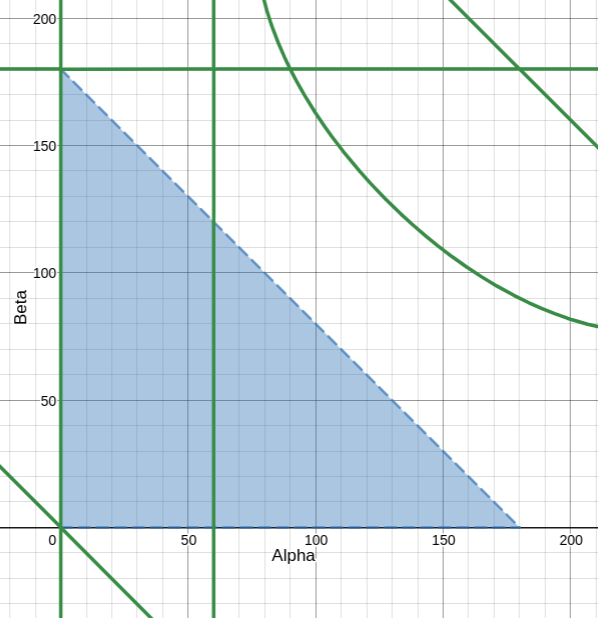
\includegraphics[width=5in]{media/R2P5Solutions.png}
        \caption{Graph outputted by Desmos for above input}
    \end{figure}
    
    Therefore, we have proved that
    \begin{equation*}
        PO\perp OI_A \implies \alpha=60^\circ. \tag*{\qed}
    \end{equation*}
    
\end{solution}

\end{document}